% This file was created by matplotlib2tikz v0.6.16.
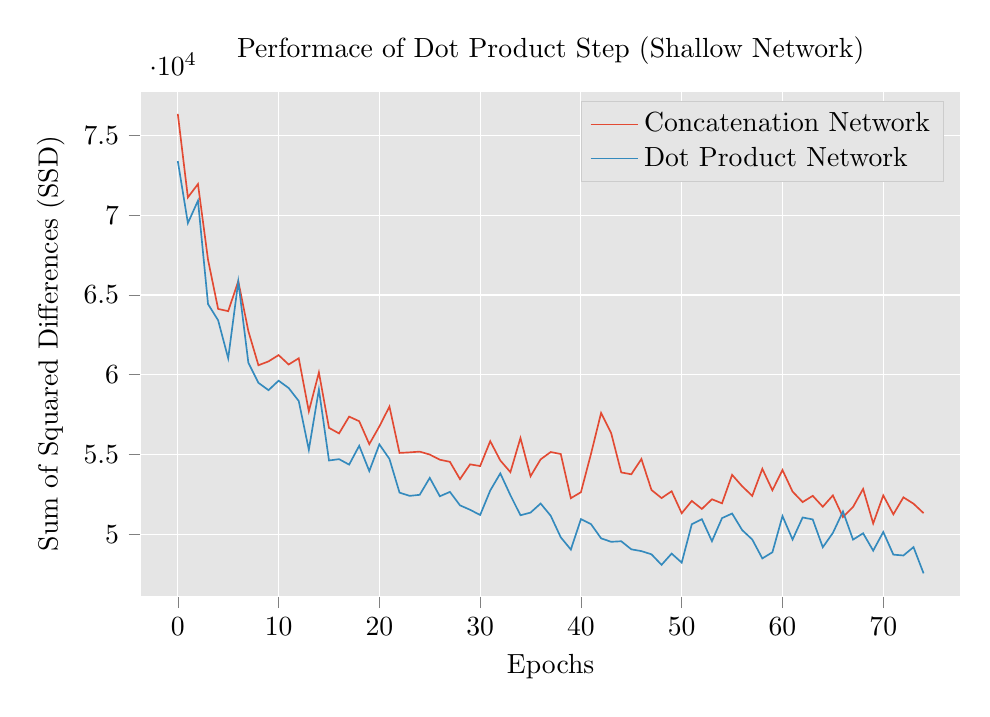
\begin{tikzpicture}

\definecolor{color1}{rgb}{0.203921568627451,0.541176470588235,0.741176470588235}
\definecolor{color0}{rgb}{0.886274509803922,0.290196078431373,0.2}

\begin{axis}[
title={Performace of Dot Product Step (Shallow Network)},
xlabel={Epochs},
ylabel={Sum of Squared Differences (SSD)},
xmin=-3.7, xmax=77.7,
ymin=46100.3080078125, ymax=77792.5240234375,
width=12cm,
height=8cm,
tick align=outside,
tick pos=left,
xmajorgrids,
x grid style={white},
ymajorgrids,
y grid style={white},
axis line style={white},
axis background/.style={fill=white!89.80392156862746!black},
legend entries={{Concatenation Network},{Dot Product Network}},
legend style={draw=white!80.0!black, fill=white!89.80392156862746!black},
legend cell align={left}
]
\addlegendimage{no markers, color0}
\addlegendimage{no markers, color1}
\addplot [semithick, color0]
table {%
0 76351.96875
1 71117.0546875
2 71955.4609375
3 67205.3203125
4 64124.5625
5 63982.953125
6 65862.359375
7 62730.09765625
8 60590.8125
9 60832.90625
10 61228.30859375
11 60637.75
12 61030.08984375
13 57703.96875
14 60139.66796875
15 56665.75390625
16 56316.37109375
17 57370.06640625
18 57081.84375
19 55645.140625
20 56757.48828125
21 57998.80078125
22 55093.46484375
23 55129.10546875
24 55174.828125
25 54991.52734375
26 54667.546875
27 54535.46484375
28 53449.65625
29 54377.41015625
30 54269.484375
31 55830.96484375
32 54619.46875
33 53889.08203125
34 56029.55078125
35 53631.953125
36 54689.28515625
37 55150.22265625
38 55024.390625
39 52253.77734375
40 52631.890625
41 55037.73828125
42 57601.19140625
43 56334.703125
44 53869.78125
45 53753.93359375
46 54711.68359375
47 52770.390625
48 52262.109375
49 52690.29296875
50 51312.76953125
51 52084.48828125
52 51580.90234375
53 52188.34765625
54 51933.05859375
55 53719.30078125
56 53002.00390625
57 52400.02734375
58 54097.60546875
59 52750.41015625
60 54018.41015625
61 52669.06640625
62 52010.19140625
63 52403.515625
64 51717.859375
65 52430.33984375
66 51069.22265625
67 51704.84375
68 52835.58203125
69 50671.625
70 52429.33203125
71 51243.26953125
72 52308.34375
73 51909.51171875
74 51317.17578125
};
\addplot [semithick, color1]
table {%
0 73394.546875
1 69506.5234375
2 70909.7890625
3 64425.296875
4 63411.30078125
5 61028.50390625
6 65840.78125
7 60750.09375
8 59488.41796875
9 59028.65234375
10 59623.71875
11 59163.08203125
12 58349.31640625
13 55292.046875
14 59072.578125
15 54618.953125
16 54703.67578125
17 54359.640625
18 55541.76171875
19 53957.76171875
20 55630.640625
21 54717.109375
22 52605.16796875
23 52400.73046875
24 52465.71484375
25 53529.859375
26 52373.50390625
27 52651.0625
28 51805.91015625
29 51528.87890625
30 51200.26953125
31 52736.30859375
32 53810.796875
33 52444.37890625
34 51184.08203125
35 51351.953125
36 51920.33984375
37 51156.234375
38 49801.25390625
39 49032.63671875
40 50942.35546875
41 50627.05078125
42 49738.62109375
43 49519.57421875
44 49555.26953125
45 49047.65234375
46 48936.09765625
47 48735.796875
48 48074.16796875
49 48781.09765625
50 48215.35546875
51 50621.68359375
52 50941.546875
53 49557.98828125
54 51005.703125
55 51293.96484375
56 50254.953125
57 49663.81640625
58 48477.23828125
59 48866.15234375
60 51133.48828125
61 49662.11328125
62 51046.66015625
63 50923.33203125
64 49177.34375
65 50078.453125
66 51422.77734375
67 49656.375
68 50053.5625
69 48965.765625
70 50135.90625
71 48715.640625
72 48661.94140625
73 49186.546875
74 47540.86328125
};
\end{axis}

\end{tikzpicture}